\documentclass{beamer}
\usepackage[utf8]{inputenc}

\usetheme{Madrid}
\usecolortheme{default}
\usepackage{amsmath,amssymb,amsfonts,amsthm}
\usepackage{txfonts}
\usepackage{tkz-euclide}
\usepackage{listings}
\usepackage{adjustbox}
\usepackage{array}
\usepackage{tabularx}
\usepackage{gvv}
\usepackage{lmodern}
\usepackage{circuitikz}
\usepackage{tikz}
\usepackage{graphicx}

\setbeamertemplate{page number in head/foot}[totalframumber]

\usepackage{tcolorbox}
\tcbuselibrary{minted,breakable,xparse,skins}



\definecolor{bg}{gray}{0.95}
\DeclareTCBListing{mintedbox}{O{}m!O{}}{%
  breakable=true,
  listing engine=minted,
  listing only,
  minted language=#2,
  minted style=default,
  minted options={%
    linenos,
    gobble=0,
    breaklines=true,
    breakafter=,,
    fontsize=\small,
    numbersep=8pt,
    #1},
  boxsep=0pt,
  left skip=0pt,
  right skip=0pt,
  left=25pt,
  right=0pt,
  top=3pt,
  bottom=3pt,
  arc=5pt,
  leftrule=0pt,
  rightrule=0pt,
  bottomrule=2pt,
  toprule=2pt,
  colback=bg,
  colframe=orange!70,
  enhanced,
  overlay={%
    \begin{tcbclipinterior}
    \fill[orange!20!white] (frame.south west) rectangle ([xshift=20pt]frame.north west);
    \end{tcbclipinterior}},
  #3,
}
\lstset{
    language=C,
    basicstyle=\ttfamily\small,
    keywordstyle=\color{blue},
    stringstyle=\color{orange},
    commentstyle=\color{green!60!black},
    numbers=left,
    numberstyle=\tiny\color{gray},
    breaklines=true,
    showstringspaces=false,
}
%------------------------------------------------------------
%This block of code defines the information to appear in the
%Title page
\title %optional
{9.4.14}
\date{October 3,2025}
%\subtitle{A short story}

\author % (optional)
{EE25BTECH11002 - Achat Parth Kalpesh}



\begin{document}

\frame{\titlepage}

\begin{frame}{Question}
Find the roots of the following quadratic equations graphically
\begin{align}
    \brak{x-3}\brak{2x-1}=x\brak{x+5}
\end{align}
\end{frame}

\begin{frame}{Theoretical Solution}
\begin{align}
    y = \brak{x-3}\brak{2x-1}-x\brak{x+5} = 0\\
    y = x^2 - 12x + 3 = 0
\end{align}
This quadratic can be represented as a conic in matrix form:
\begin{align}
   \vec{x}^{\top}\vec{V}\vec{x} + 2\vec{u}^{\top}\vec{x} + f = 0\\ 
   \vec{V} = \myvec{1 & 0 \\ 0 & 0} , \vec{u} = \myvec{-6 \\0} ,
   f = 3
\end{align}
To find the roots, we find the points of intersection of the conic with the x-axis.
\begin{align}
\vec{x} = \vec{h} + k_i\vec{m}    
\end{align}
\begin{align}
\vec{h}=\myvec{0 \\ 0}, \vec{m} = \myvec{1 \\ 0}
\end{align}
\end{frame}


\begin{frame}{Theoretical Solution}
The value of $k_i$ can be found out by solving the line and conic equation

\begin{align}
\brak{\vec{h} + k_i \vec{m}}^{\top} \vec{V} \brak{\vec{h} + k_i \vec{m}} + 2\vec{u}^{\top} \brak{\vec{h} + k_i \vec{m}} + f &= 0 \\
\implies k_i^{2} \vec{m}^{\top}\vec{V}\vec{m} + 2k_i \vec{m}^{\top} \brak{\vec{V}\vec{h} + \vec{u}} + \vec{h}^{\top}\vec{V}\vec{h} + 2\vec{u}^{\top}\vec{h} + f &= 0 \\
\text{or, } k_i^{2} \vec{m}^{\top}\vec{V}\vec{m} + 2k_i \vec{m}^{\top} \brak{\vec{V}\vec{h} + \vec{u}} + g\brak{\vec{h}} &= 0
\end{align}

Solving the above quadratic gives the equation
\begin{align}
k_i = \frac{1}{\vec{m}^{\top}\vec{V}\vec{m}}
\brak{
    -\vec{m}^{\top} \brak{\vec{V}\vec{h} + \vec{u}}
    \pm
    \sqrt{ \sbrak{\vec{m}^{\top}\brak{\vec{V}\vec{h} + \vec{u}}}^2
    - g\brak{\vec{h}} \ \brak{\vec{m}^{\top}\vec{V}\vec{m}} }
    }
\end{align}
\end{frame}

\begin{frame}{Theoretical Solution}
Substituting the values in the above equation gives
\begin{align}
\therefore k_i =6 \pm \sqrt{33}
\end{align}
\begin{align}
 k_1 = 6 + \sqrt{33}\\
 k_2 = 6 - \sqrt{33}
\end{align}
\begin{align}
    \vec{x} = \vec{h} + k_i\vec{m}
   = \myvec{6 + \sqrt{33} \\ 0},\quad
     \myvec{6 - \sqrt{33} \\ 0}
\end{align}
\end{frame}
\begin{frame}[fragile]
    \frametitle{C code}
    \begin{lstlisting}
#include <stdio.h>
#include <math.h>

double root1(double a, double b, double c) {
    double d = b*b - 4*a*c;
    return (-b + sqrt(d)) / (2*a);
}

double root2(double a, double b, double c) {
    double d = b*b - 4*a*c;
    return (-b - sqrt(d)) / (2*a);
}
    \end{lstlisting}
\end{frame}

\begin{frame}[fragile]
    \frametitle{Python Code}
    \begin{lstlisting}[language=Python]
import numpy as np
import matplotlib.pyplot as plt
import ctypes

lib = ctypes.CDLL("./formula.so")

lib.root1.argtypes = [ctypes.c_double, ctypes.c_double, ctypes.c_double]
lib.root1.restype = ctypes.c_double

lib.root2.argtypes = [ctypes.c_double, ctypes.c_double, ctypes.c_double]
lib.root2.restype = ctypes.c_double

def quadratic(a, b, c):
    x1 = lib.root1(a, b, c)
    x2 = lib.root2(a, b, c)
    return x1, x2
    \end{lstlisting}
\end{frame}
\begin{frame}[fragile]
    \frametitle{Python Code}
    \begin{lstlisting}[language=Python]
def function(x):
    return x**2 - 12*x + 3

x = np.linspace(-3, 15, 100)
y = function(x)
y1 = np.zeros(100)
x1, x2 = quadratic(1, -12, 3)
fig, ax = plt.subplots()
ax.plot(x, y, label='x^2 - 12x + 3') 
ax.plot(x, y1, label='y = 0')
ax.scatter(x1, 0, color="black", label=f'Root 1 ({x1:.2f}, 0)')
ax.text(x1, 0, f'({x1:.2f}, 0)')
ax.scatter(x2, 0, color="black", label=f'Root 2 ({x2:.2f}, 0)')
ax.text(x2, 0, f'({x2:.2f}, 0)')
ax.grid(True)
ax.legend(loc="lower right")
plt.show()
    \end{lstlisting}
\end{frame}

\begin{frame}{Plot}
    \begin{figure}
        \centering
        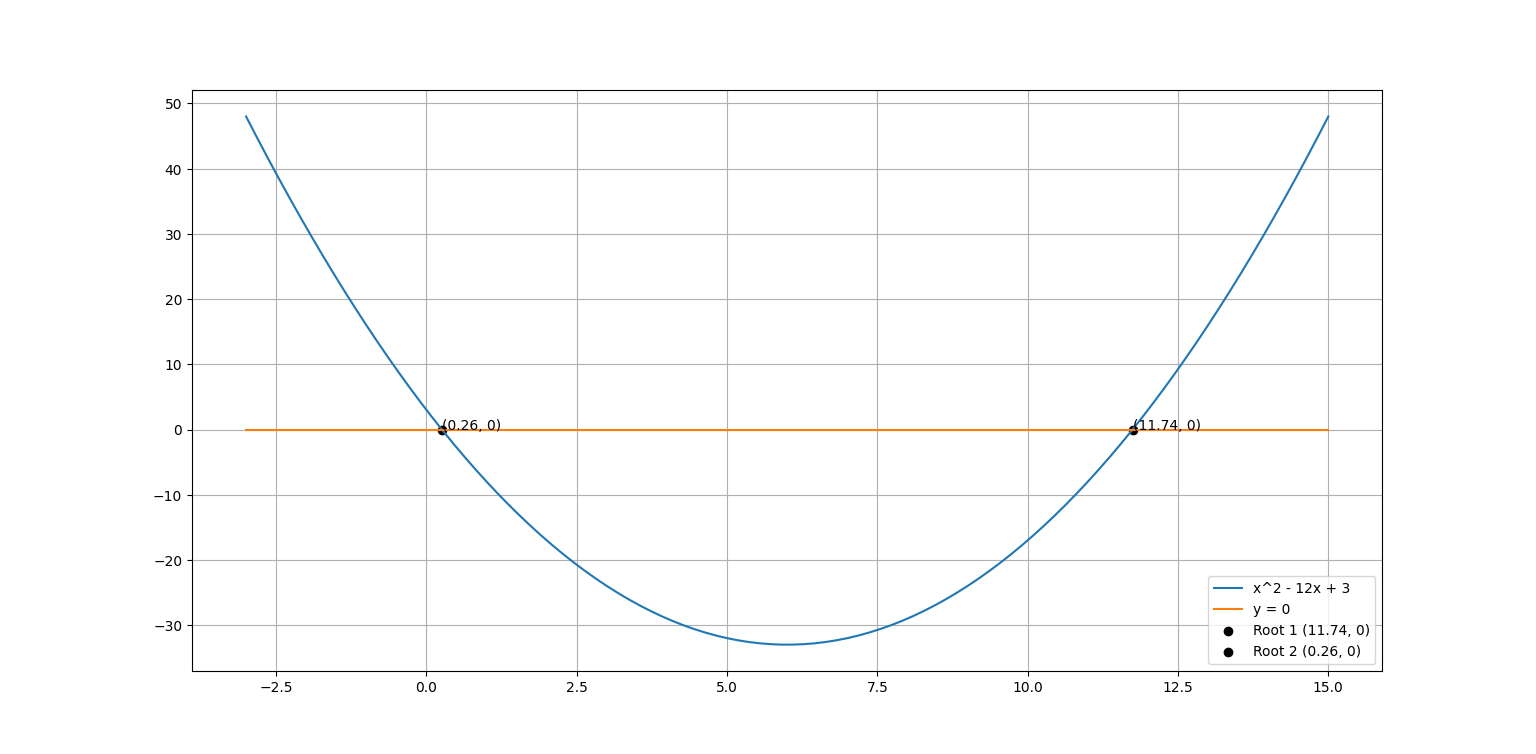
\includegraphics[width=\columnwidth]{../figs/figure_py.png}
        \caption{Graphical Representation of quadratic equation}
        \label{fig:final_plot}
    \end{figure}
\end{frame}
\end{document}
